%# -*- coding: utf-8-unix -*-
%%==================================================
%% chapter03.tex for SJTU Master Thesis
%% software requirement specification
%%==================================================
%\bibliographystyle{sjtu2}%[此处用于每章都生产参考文献]

\chapter{相似轨迹查询系统设计与实现}
\label{chap:system requirement specification}

\section{本章序言}
\label{sec:introduction}
随着相似轨迹查询这以在科研领域和工业应用中的不断发展,开发相似轨迹查询系统为用户在搜索相似轨迹中提供更方便更可视化的结果。为了明确关于相似轨迹查询系统的设计需求、应用领域与系统功能,在本章节中,本文首先对相似轨迹查询系统的设计与实现作细节说明和具体描述。我们对本章节的目的以及之后说明中会涉及到的名词概念进行解释,以便于之后章节的拓展。该系统是主要以Python进行后端数据处理,系统运行于以Python为基础的Flask Web内部依赖Werkzeurg的工作集服务器。用户只需要通过进行简单操作便可以实现个性化的相似轨迹查询操作,并了解本系统软件的基本工作原理。

\subsection{系统应用现状调查}
\label{subsec:application situation}
目前相似轨迹查询这一领域的研究成果在学术方面有着丰富和较为系统的成果,不过目前这些学术成果移植到系统应用中的样例较为稀缺。在国内开发的地图应用或者提供以地图搜索为主体的公司在相似轨迹查询这一领域所投入的精力并不多,导致基于相似轨迹查询的系统软件发展投入在实际应用中的比例相对较少。

\subsection{系统应用范围}
\label{subsec:scope}
相似轨迹查询系统是一个基于\emph{GPS}轨迹数据的服务器端应用系统。根据轨迹用户提供的输入轨迹或一组基于GPS数据的轨迹点集,系统帮助用户在地理语义上查询出与输入最相似的k条结果轨迹。系统可以免费从Github上下载并运行在可以运行Python程序的平台上。

本系统在应用中,需要连接互联网以调用基于Javascript的地图服务接口,实现地图显示和轨迹显示等等基础功能。所有系统所需要的轨迹数据以文件系统存储于服务器端。在系统运行过程中,用户可以通过浏览器登录页面进行系统访问,结合用户自身查询需求系统得出不同的查询结果。本系统也支持展示出所有地图上具体位置信息和查询具体地理位置的功能。

\subsection{读者对象}
\label{subsec:target}
本章节可作为系统设计人员、系统测试人员、系统使用用户的参考资料与文档。

\subsection{编写原则}
\label{subsec:principle}
\begin{itemize}
	\item 准确性:本章节所描述的针对系统的需求,设计系统的功能与行为与目标软件系统产品实现期望相符。
	\item 完整性:包括全部有实际应用意义的系统需求,在功能、性能和设计方面均满足所需的需求。依照《系统软件设计规范说明书》的要求,将描述系统需求所需的流程图和名词定义给出完整描述。
	\item 易读性:本章节内容通过简要文字,辅以插图和图标,让读者对象能够清楚了解系统设计中的需求内容。
	\item 可验证性:对于本章节中所编写的系统需求分析与设计内容,读者可通过实际系统进行功能、性能和设计方面上的检查以校对是否与编写内容一致。
\end{itemize}

\subsection{系统名词定义}
\label{subsec:definitions}
表\ref{tab-system definitions}所示。
\begin{table}[!htpb]
  	\centering
		\begin{tabular}{ |p{3cm}||p{9cm}|  }
		\hline
		符号标记 & 符号注释 \\
		\hline
		用户 & 使用相似轨迹查询系统进行轨迹查询人员 \\
		\hline
		管理员 & 相似轨迹查询系统管理员,负责运行权限和控制系统 \\
		\hline
		轨迹数据 & 移动物体上空间上按时间顺序的移动数据记录 \\
		\hline
		GPS & 全球定位系统 \\
		\hline
		DESC & 描述 \\
		\hline
		DEP & 依赖 \\
		\hline
		\end{tabular}
	\bicaption[tab-system definitions]{相似轨迹查询系统涉及名词定义}{相似轨迹查询系统涉及名词定义}{Table}{A list of definitions and explanations in the system of searching similar trajectories}
\end{table}

\section{系统设计需求分析}
\label{sec:overall description}
在开展相似轨迹查询系统设计之前,我们首先对要设计的系统所涉及的实际需求进行描述。在定义好该系统所需要解决的应用问题和需要满足的用户需求之后,在因地制宜设计系统框架。

\subsection{系统需求概述}
\label{subsec:general requirements}
随着GPS技术不断发展和私家车数量的激增,生活中每天都会产生海量数据规模的轨迹数据。用户想要根据特定需求查询轨迹(例如本文所要解决的查询相似轨迹),通过传统的软件系统难以高效查询出所期望的结果。我们通过基于目前主流的算法实现,设计出快速、准确的相似轨迹查询系统,借助网页地图接口将查询结果清晰了然展示在用户界面上。系统在实现相似轨迹查询的基础上,可以为用户提供轨迹路径规划和轨迹推荐等基于相似轨迹查询的应用服务。

\subsection{系统需求说明目的}
\label{subsec:propose}
在完成对相关工作的研究和系统市场的前景分析后,本文提出相似轨迹查询系统设计需求说明。相似轨迹查询查询系统设计需求说明的目的在于对于本系统进行具体描述,明确索要开发的系统应该具备的功能与界面,为系统分析及移植开发提供清晰的基础需求描述,并以此为基础进一步满足后续设计与开发。本文所设计开发的相似轨迹查询系统目标是为用户提供高效、准确的查询服务平台。系统针对目前轨迹信息管理的实际情景,较为全面地满足用户的查询需求,初步实现系统所制定的设计初衷。需求说明从字面上作为软件系统发展的指导和完备部分,解释说明了系统中的限制条件、应用交互接口以及具体功能。


\subsection{用户功能需求}
\label{subsec:user class functional requirements}
\begin{enumerate}
   \item 一般查询用户:
   \begin{itemize}
   		\item 基于轨迹点集的相似轨迹查询功能:一般查询用户在地图界面上点击地理位置或根据查询输入窗口输入查询地点,同时可以增加或删除查询点。查询轨迹点集会以小图标的形式显示上地图上。结合查询日期条件,搜索出相似轨迹。
   \end{itemize}
   \item 登录用户:
   \begin{itemize}
		\item 登录功能:登录用户ID和密码登录到用户界面,显示用户的历史轨迹。
		\item 显示历史轨迹数据功能:登录用户可以选择一条历史轨迹数据,展示与地图上
		\item 基于历史轨迹的相似轨迹查询功能:在选择一条历史轨迹时候,登录用户在设定好查询时间参数后可以进行相似轨迹查询功能。
		\item 基于轨迹点集的相似轨迹查询功能:一般查询用户在地图界面上点击地理位置或根据查询输入窗口输入查询地点,同时可以增加或删除查询点。查询轨迹点集会以小图标的形式显示上地图上。结合查询日期条件,搜索出相似轨迹。
   \end{itemize}
\end{enumerate}

\subsection{用户界面需求}
\label{subsec:external interface Requirements}
\begin{itemize}
	\item 用户登录界面:实现用户账户与密码登录。
	\item 功能选择界面:进入相似轨迹查询系统后选择用户所需要的功能。
	\item 地图显示界面:在一般用户和登录用户模式中都可以显示城市地图信息,通过高德地图\cite{AutoNavi}接口实现附属界面功能。
	\item 地理位置点输入界面:在输入界面中输入地址位置名称,显示对应的地理经纬度坐标并在地图上显示具体位置。
	\item 查询条件设定界面:相似轨迹查询窗口,结合用户自定义条件作为相似轨迹查询的附属输入参数。
	\item 历史轨迹显示界面:显示登录用户的历史轨迹数据条目。
\end{itemize}

%%%%%%%%%%%%%%%%%%%%

\section{系统设计}
\label{sec:overall description}
本文设计的相似轨迹查询系统运行运行于基于Python语言的Flask Web框架,运行过程中需要连接互联网以使用地图接口,系统内部数据为上海私家车数据。系统针对的用户为一般用户和登录用户。一般用户可以目的轨迹点集进行相似轨迹查询,实现路径规划等具体应用,用户在运用过程中需要在地图上点击位置以实现轨迹点击输入;登录用户在一般用户具有功能基础上,用户的历史轨迹在轨迹数据库中有存储,可以实现以一条轨迹为输入的相似轨迹查询,实现拼车或轨迹推荐等具体应用。本系统目前已有依赖于Flask框架和地图接口提供。

\subsection{系统设计框架}
\label{subsec:product perspective}
相似轨迹查询系统主要由前后端两部分组成。后端部分主要以轨迹预处理、相似轨迹查询和查询请求分析处理为主;前端以部分地图轨迹可视化、查询结果输出、地理位置搜索等部分组成。

针对相似轨迹查询系统的后端处理流程思路主要为,在后台运行服务器代码,接收来自浏览器前端的请求。将请求分析与提前预先设定的资源定位符函数结合,对于数据类型选择是否进行轨迹数据预处理。针对同一的输入轨迹数据点集,进行相似轨迹数据查询功能服务。然后将结果作为请求返回返回给用户。实现一次相似轨迹查询请求过程。与此同时,系统前端主要以实现数据可视化为主,以一个窗口形式将地图数据显示。对于用户感兴趣的地理位置坐标点和历史轨迹数据,可以通过点击地图或历史轨迹数据项目将数据在地图窗口上得以可视化展示。

\begin{figure}[!htp]
  \centering
  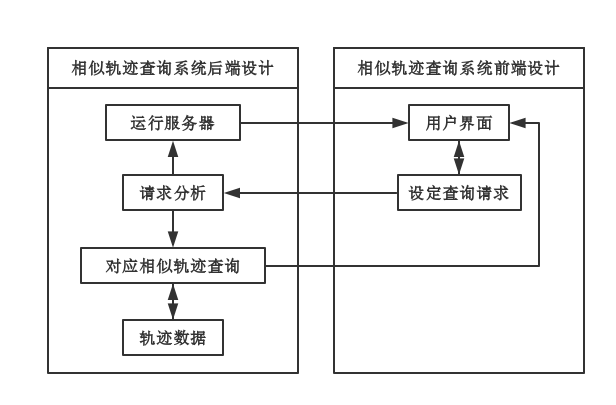
\includegraphics[width=0.8\textwidth]{specification/system-architecture.png}
  \bicaption[fig:system-architecture]{相似轨迹查询系统设计框架}{相似轨迹查询系统设计框架}{Fig}{System design architecture}
\end{figure}

\subsection{系统功能描述}
\label{subsec:product functions}
在相似轨迹查询系统中,一般用户和登录用户都可以使用相似轨迹查询功能。查询结果与用户定义的输入轨迹数据类型(为轨迹点集或一条历史轨迹)、查询的日期、相似轨迹数目阈值和查询是否有序性有关。

相似轨迹查询的主要是通过在地图上以不同颜色和不同粗细的折线端进行表示。在查询结果中,根据与查询输入相似度的相关性,越相似的查询结果轨迹将以越显著的参数表示出来,用户可以一目了然在地图上得出最符合查询的结果的一条或多条轨迹。

\subsection{系统运行环境}
\label{subsec:system environment}

表\ref{tab-system environments}对本系统运行环境进行了描述。
\begin{table}[!htpb]
  	\centering
		\begin{tabular}{ |p{1cm}|p{3.5cm}|p{8.5cm}| }
		\hline
		序号 & 环境需求 & 环境参数 \\
		\hline
		01 & 系统操作系统 & Mac OS 10.11.6  \\
		\hline
		02 & 分布式操作系统 & Ubuntu14.04.1 amd64  \\
		\hline
		03 & 单机PC设备参数 & 处理器 2.6 GHz Intel Core i5且内存大于等于4G\\
		\hline
		04 & 分布式PC设备参数 & 处理器 2.6 GHz Intel Core i5且内存大于等于1G\\
		\hline
		05 & 服务器平台 & Flask0.12/Python2.7.6 \\
		\hline
		\end{tabular}
	\bicaption[tab-system environments]{相似轨迹查询系统运行环境}{相似轨迹查询系统运行环境}{Table}{A list of environment parameters in the system of searching similar trajectories}
\end{table}

\subsection{用户类与特点}
\label{subsec:user characteristics}
相似轨迹查询系统的使用者主要分为轨迹查询用户和管理用户。

对于轨迹查询用户而言,我们通过是否具有在系统中存储这历史轨迹数据分为登录用户和一般用户。一般用户是系统的流动用户,在系统轨迹数据库中不具备历史轨迹。一般用户只能通过向系统输入一组轨迹查询点集以完成相似轨迹查询功能。登录用户可以根据账户信息和密码登录相似轨迹查询系统,使用已有的历史轨迹数据或是自定义的一组轨迹点集实现相似轨迹查询功能。

相似轨迹查询系统中的管理员主要负责登录用户的权限管理和对历史数据的修改处理操作。管理员对于相似轨迹查询系统中违反查询和使用规范的用户可以修改其登录权限以阻止其进一步违规操作。管理员还可以对历史轨迹进行增加、修改和删除操作,以保证系统数据库的实时性和准确性。

\subsection{系统处理流程}
图\ref{fig:system-flowchart}展示了相似轨迹查询系统的主要流程。进入相似界面之后,用户可以直接使用系统(即不需要登录)使用系统进行相似轨迹查询,在获取满意的查询结果之后退出系统。同时,如果需要运用登录功能,系统会在登录界面中提醒用户是选择轨迹历史用户登录还是管理员模式登录。对于轨迹历史用户,可以实现相对应的轨迹查询类型并和一般用户一样在得到满意的查询结果之后退出系统。对于管理员而言,他们主要负责对用户权限和轨迹数据处理这一部分工作,在完成管理员工作之后他们也可以按流程退出系统。

\label{subsec:system flow}
\begin{figure}[!htp]
    \centering
    \resizebox{14cm}{!}{
\begin{tikzpicture}[node distance=2cm]

	%\node (input) [startstop] {输入轨迹数据类型判断};
	%\node (input_judge) [decision, below of=input,yshift=-0.5cm,aspect=2.5] {是否为用户指定一组轨迹点集?};
	%\node (ts) [process, right of=input_judge,xshift=5cm] {轨迹简化};
	%\node (iknn) [process, below of=input_judge,yshift=-0.5cm]{增长型k相似轨迹查询};
	%\node (bound_judge) [decision, below of=iknn,yshift=-0.5cm,aspect=2.5]{是否满足相似度上下界条件?};
	%\node (refinement)[process, below of=bound_judge,yshift=-0.5cm]{备选轨迹集筛选};
	%\node (output)[startstop, below of=refinement]{k条最相似轨迹输入};
	

%	\draw [arrow] (input) -- (input_judge);
%	\draw [arrow] (input_judge) -- node[anchor=south]{否}(ts);
%	\draw [arrow] (input_judge) -- node[anchor=west]{是}(iknn);
%	\draw [arrow] (ts) |- (iknn);
%	\draw [arrow] (iknn) -- (bound_judge);
%	\draw [arrow] (bound_judge.west) |- node[anchor=south]{否}(iknn.west);
%	\draw [arrow] (bound_judge.south) -- node[anchor=west]{是}(refinement.north);
%	\draw [arrow] (refinement) -- (output);

	\node (begin) [startstop,font=\bf,fill=green!20] {进入系统界面};
	\node (login_judge) [decision, below of=begin, yshift=-0.5cm, aspect=2.5]{是否需要登录};
	\node (general) [process, right of=login_judge, xshift=3cm]{一般用户};
	\node (login_type_judge) [decision, below of=login_judge, yshift=-0.5cm, aspect=2.5]{是否为管理员};
	\node (history) [process, right of=login_type_judge, xshift=3cm]{登录用户};
	\node (admin) [process, below of=login_type_judge]{管理员操作};
	\node (search) [process, right of=history, xshift=3cm]{相似轨迹查询};
	\node (is_search_good) [decision, below of=search, aspect=2.5]{是否满意查询结果};
	\node (does_admin_finish) [decision, below of=admin, aspect=2.5]{管理员操作是否完成};
	\node (finish) [process, below of=history]{系统处理完成};
	\node (stop) [startstop, below of=finish,font=\bf,fill=green!20]{退出系统界面};
	
	
	
	\draw [arrow](begin.south) -- (login_judge.north);
	\draw [arrow](begin.east) -| node[anchor=south]{直接查询模式}(general.north);
	\draw [arrow](login_judge.east) -- node[anchor=north]{否}(general.west);
	\draw [arrow](login_judge.south) -- node[anchor=west]{是}(login_type_judge.north);
	\draw [arrow](login_type_judge.east) -- node[anchor=north]{否}(history.west);
	\draw [arrow](login_type_judge.south) -- node[anchor=west]{是}(admin.north);
	\draw [arrow](general.east) -| (search.north);
	\draw [arrow](history.east) -- (search.west);
	
	\draw [arrow](search.south) -- (is_search_good.north);
	\draw [arrow](is_search_good.east) |- node[anchor=west]{否}(search.east);
	\draw [arrow](is_search_good.west) -- node[anchor=north]{是}(finish.east);
	
	\draw [arrow](admin.south) -- (does_admin_finish.north);
	\draw [arrow](does_admin_finish.west) |- node[anchor=east]{否}(admin.west);
	\draw [arrow](does_admin_finish.east) |- node[anchor=east]{是}(finish.west);
	
	\draw [arrow](finish.south) -- (stop.north);

\end{tikzpicture}

}
    \bicaption[fig:system-flowchart]{相似轨迹查询系统处理流程图}{相相似轨迹查询系统处理流程图}{Fig}{A flow chart of searching similar trajectory system}
\end{figure}


\section{系统分析}
\label{sec:system analysis}

\subsection{系统组成分析}
\label{subsec:component analysis}

\subsection{系统性能分析}
\label{subsec:performance analysis}

